\section{Recurring Failure as a Missing Procedure}
\label{sec:mechanism}
Let a scenario generate a sequence of release periods $t_1,\ldots,t_K$. At each period, the agent receives a cutoff-valid evidence state $E_t$ and a question $x_t$. The agent also carries a reusable skill library $L_t$. Future behavior follows
\begin{equation}
Y_t = H(x_t,E_t,L_t,S_t),
\end{equation}
where $S_t$ contains the remaining agent state.

A recurring failure mode appears when the same procedural error repeats across periods while the concrete evidence changes. This pattern suggests that the agent lacks a reusable operation. We represent the missing operation as a skill $g_m$ associated with mechanism $m$.

\begin{figure}[t]
\centering
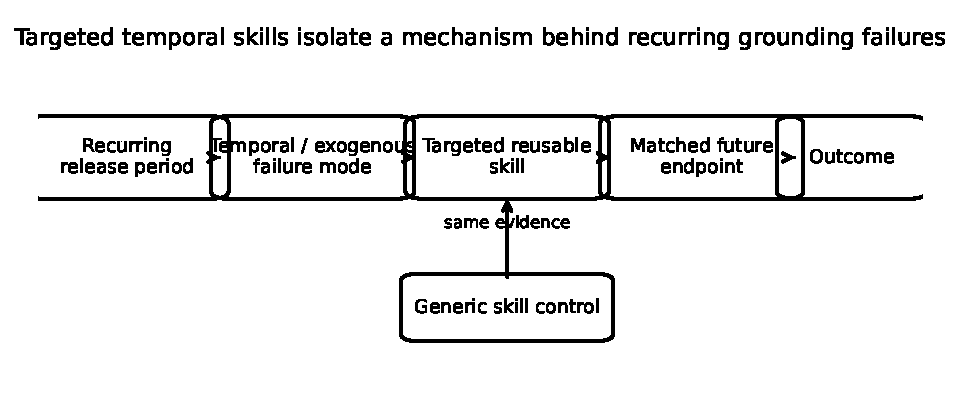
\includegraphics[width=\linewidth]{figures/fig1_temporal_skill_causal.pdf}
\caption{Targeted skill intervention. The same future endpoint is evaluated with a mechanism-specific skill and with a matched generic skill. This isolates the contribution of the procedure encoded by the targeted skill.}
\label{fig:causal}
\end{figure}

The causal estimand compares outcomes on the same future endpoint under two skill libraries:
\begin{equation}
\Delta_m =
\mathbb{E}[Y_t\mid do(L_t=L\cup\{g_m\})]-
\mathbb{E}[Y_t\mid do(L_t=L\cup\{g_c\})],
\end{equation}
where $g_c$ is a generic control skill with matched implementation complexity. A positive $\Delta_m$ supports the claim that the target procedure repairs the matched failure beyond generic skill assistance.

\subsection{Temporal cutoff skill}
The cutoff skill receives a query date and a set of candidate evidence timestamps. It returns the admissible evidence subset under the benchmark cutoff. Its purpose is to prevent later releases from leaking into earlier-period analysis. The skill can also expose the cutoff date explicitly to subsequent reasoning.

\subsection{Release alignment skill}
The alignment skill maps source-release dates to the benchmark period represented by the evidence. It is useful when the source publication date differs from the underlying reporting period. The skill returns a normalized period identifier and verifies that the selected time-series row matches that period.

\subsection{Exogenous grounding skill}
The grounding skill links a numerical change to documentary evidence available before the cutoff. It searches prior-period reports for candidate events and returns evidence spans tied to the target period. This procedure supports attribution questions that require context outside the numerical series.

Each skill encodes a reusable operation that excludes scenario-specific answers. The same function can apply across future periods. This property matches the source harness contract for skills saved through \texttt{induct\_skill}.
